%equations, bib. \\

\section{Literature Review}

\noindent This chapter will examine the current literature and research related to different methods of scanning, advantages and disadvantages, weak points and strength of each method. Methods mainly  consists of 360 degree scanning, photogrametry, Lidar with a sample used case for ship damage assessment, NeRF and 3D Gaussian Splatting for scanning and photo-realistic 3D models. For Aerial-based or ground-based robot scanning equipped with 360 degree camera, concepts of slam and visual slam is crucial which mentioned in this study for further work and not as a used case in my methodology. Final section of this chapter is about variety of segmentation methods for image, video and point cloud which is important specially for robot-based scanning. 
\subsection{Shipbuilding processes related to 2D and 3D modeling}
The development of large and complicated products such as ships, ferries, and offshore boats is a lengthy process that encompasses all activities till product delivery (conceptual design phase, construction and assembly phase, etc.).  Life cycle management is a difficult challenge for maritime transportation vehicles, which have long lifespans (more than 15 to 20 years) and a variety of operational conditions \cite{Favi2018}. \\ An overview of shipbuilding processes which related to 2D and 3D modeling of a ship: \\
\textbf{1. Conceptual Design:}  This phase consists of the initial ideation and drawing of the ship's design, with an emphasis on its intended purpose, capabilities, and overall attributes. In this phase possible to define the vessel's general characteristics and measurements, as well as outline requirements. For this phase designer company could develop precise general arrangement drawings, reuse current designs and previously created projects, make diagrams, and pinpoint the major equipment \cite{Favi2018}.\\
\textbf{2. Basic Design:} This phase involves comprehensive planning and design refinement, as well as detailed drawings and specifications \cite{Favi2018}. The basic design incorporates the hull form, general arrangements, needs, and other information from the initial design to create a fully working vessel. This encompasses an initial design of the structure for all crucial sections, a comprehensive analysis of the structure, designs for functional machinery and systems, space distribution for key systems, preliminary lists and specifications of equipment, models for estimating weight, and drawings approved by the class.”. To meet the industry's stringent design timetables, all team members must collaborate, from structural designers to those in charge of assigning space for critical systems. When everyone understands the implications of a change, it is simple to respond before problems occur. It also informs the entire team about progress, other essential elements such as weight management, and both intra and inter-disciplinary conflicts in the project\cite{Thedesignphase}.\\
\textbf{3. Detailed Design :}
In-depth engineering effort to complete the ship's design for construction. Even before the basic design's class approval package is granted, work is underway to add the detail required to source material, plan the construction, and drive fabrication and assembly of the vessel in the yard. This effort marks the start of the comprehensive design and will continue until the vessel is completed and ready for launch. It is crucial that this work represents a natural extension of the original idea. It is also critical that the engineering team respond promptly and efficiently to change requests, whether they come from class society comments if the basic design has not yet been authorized, production concerns, or unforeseen changes in equipment or material \cite{Thedesignphase}.\\
\textbf{4. Manufacturing and Assembly :}
Even a little shipbuilding project is massive in scope and size. Structural parts are manufactured, and interim assemblies are created specifically for that series of ships. Even within two ships in the same series, there are more differences than similarities.
For these reasons, a shipyard's deliverables are numerous, complicated, and unique to shipbuilding. The organization's design and engineering teams must be able to provide these shipbuilding deliverables while also dealing with shipbuilder-specific problems\cite{Thebuildphase}. \\
\textbf{5. Digital Twin, Maintenance and Retrofitting :}
While shipbuilding can take years, a ship will be in operation for decades, and expense distribution is the same. Even a little reduction in a ship's long-term expenditures can result in enormously huge savings when compounded over its lifetime. When the ship is turned over to the client, the digital information must stay associated with it. However, if digital data is not available, your teams must be able to gradually develop the digital twin after the event. Using technology such as laser scanning or other data collection methods to capture the vessel's on-the-water status and integrating it with any CAD, PDF, or other available data can provide your business with a comprehensive picture of the ship. Integrating data from multiple sources helps capture the intent underlying digital information and maintains the digital thread. The result is a higher ROI (Return on Invest) for boats with better-managed data. When stricter environmental standards meet longer vessel lifespans, hundreds of ships require retrofitting, maintenance, or both. Making that process as frictionless as possible, with minimal downtime, is critical to minimize the impact on a business. Every retrofit process begins with an assessment of the ship's current condition. If the ship's digital twin has not been updated throughout its career, or if the ship was built without one, the retrofit designer will most likely be unable to use existing data. This means starting from scratch but the goal is to find the most cost-effective, scalable, and efficient method of collecting on-board reality and developing adjustments without losing quality. Each retrofit project presenting unique issues and each vessel differing somewhat, using laser scanning is one method to guarantee you have as much information as possible to assist you throughout the design process \cite{LaserscanSSI,Stavroulakis2022}.

\subsection{The Role of 3D Scanning in Ship's Safety and Maintenance}
The efficiency of a ship's machinery, especially the plumbing in the engine room, is critical to its functioning and safety. The maritime sector is significantly reliant on this machinery, which affects not only the crew's lives but also the sea environment. 3D scanning technology contributes significantly to the maintenance of these systems by:\\

\textbf{1. Accurate Model Creation :} It generates comprehensive models of the engine room's pipework, allowing you to pinpoint parts that are likely to fail.\\

\textbf{2. Support of Maintenance :} The 3D models are useful references for doing inspections, repairs, and managing complex installations or retrofits.\\

\noindent 3D scan of different components in the ship can be used for inspection, reference for repairs or retrofits and complicated installation. The scanner can generate the raw data or point cloud and in the next step the technicians can make a CAD model of that components \cite{3DScan}. In Figure \ref{fig:Engine Room Scan} there are scans of engine room of a ship. 


\begin{figure}[H]
  \centering
  \subfloat[Engine Room scan in a ship]{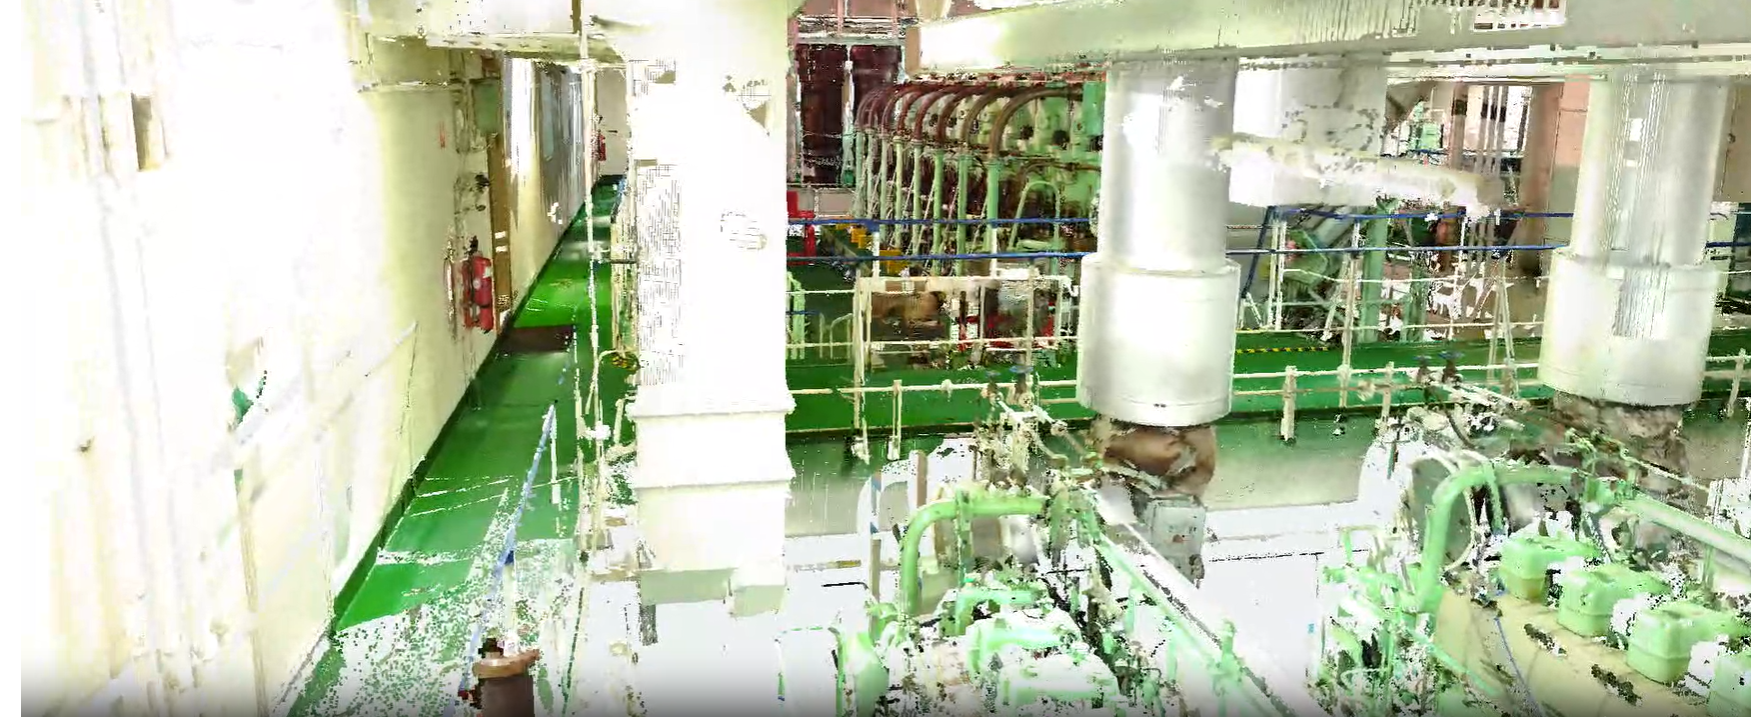
\includegraphics[width=0.9\textwidth]{Figures/EN2.png}\label{fig:Engine Room Scan}}
  \hfill
  \subfloat[Engine Room Scan 2]{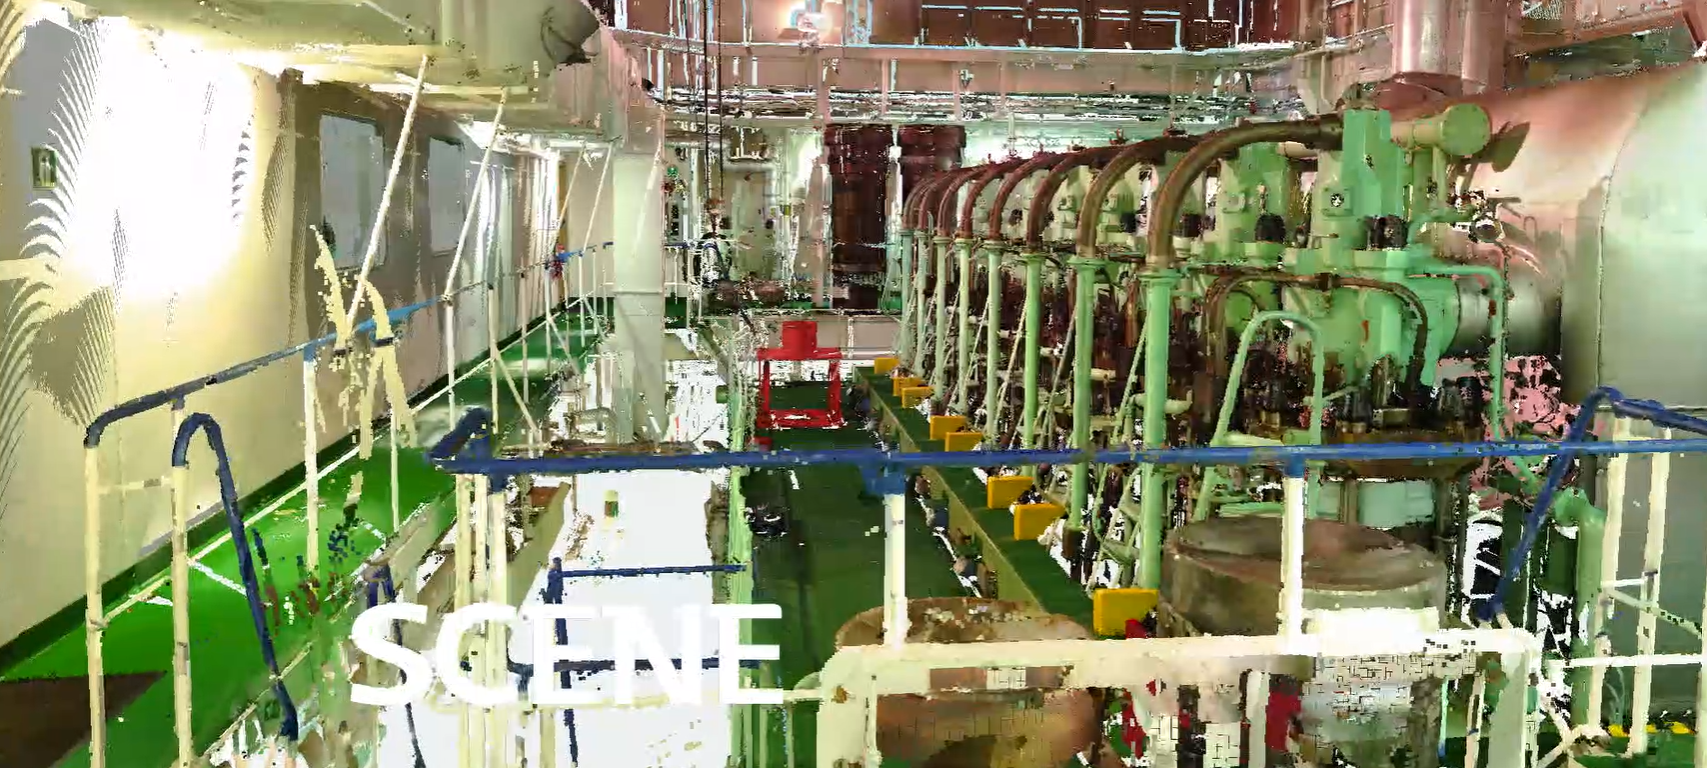
\includegraphics[width=0.9\textwidth]{Figures/ER3.png}\label{fig:Engine Room Scan 2}}
  \hfill
  \subfloat[Engine Room Scan 3]{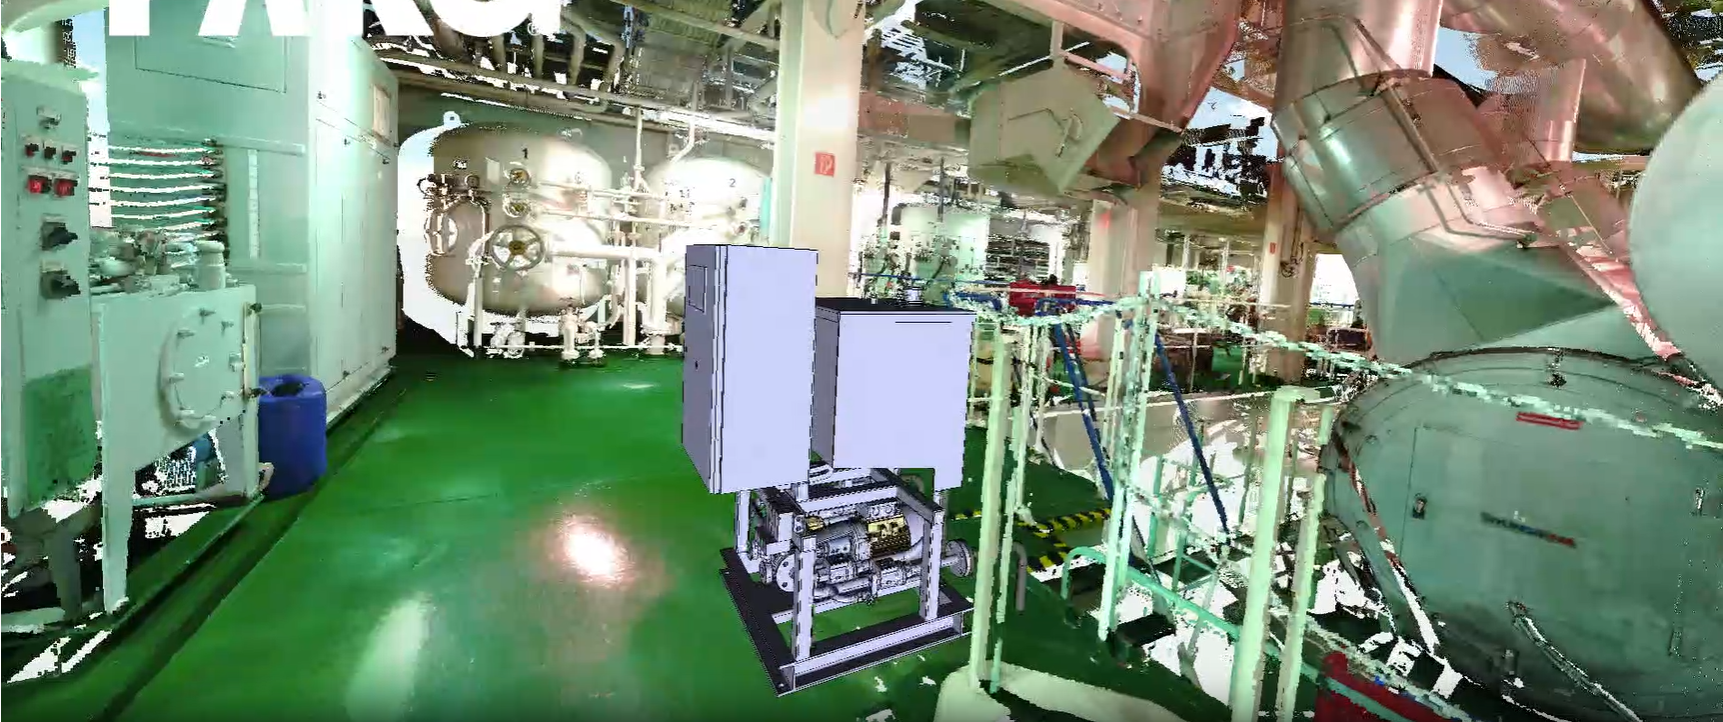
\includegraphics[width=0.8\textwidth]{Figures/ER5.png}\label{fig:Engine Room Scan 3}}
  
  \caption[Engine Room Scans from Different Views]{Figure (a) shows the point cloud from engine and pipes, figure (b) shows another view of scan in engine room, and figure (c) shows components point cloud.}
\label{fig:Engine Room scan in a Ship} \cite{3DScan}
\end{figure}

\subsubsection{Integration of Scanned Data Into the Design}
Scans of individual fabrications, modules, or as-built sites can be quickly imported and verified against the design model. 
Keep your project on track by identifying and resolving non-compliances. Use a design model that can be updated to correctly reflect the actual construction \cite{AVEVAE3D}. In the Figure \ref{fig:Laser data merge with 3D} it is shown that laser scanned equipment data are integrated with green pipes from the original 3D CAD model. 

\begin{figure}[H]
  \centering
  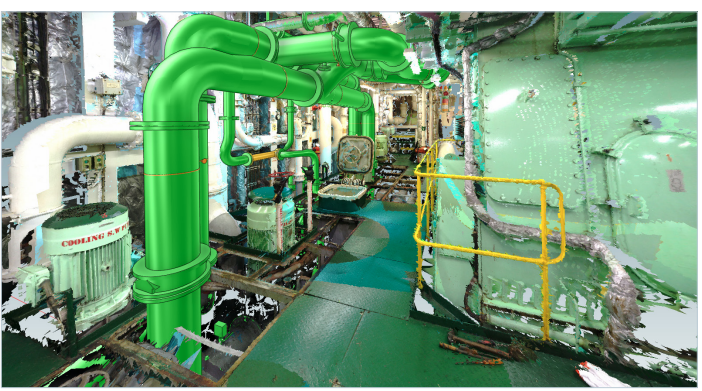
\includegraphics[width=0.9\textwidth]{Figures/AVEVAE3D.PNG}
  \caption[laser data integrated with 3D CAD model in AVEVA E3D software]{Laser scanned data merged with 3D model} \cite{AVEVAE3D}
  \label{fig:Laser data merge with 3D}
\end{figure}

\subsection{360$^{\circ}$ Camera Systems}
 This sub-chapter delves into how these 360$^{\circ}$ camera systems are used to conduct a comprehensive and complete environmental evaluation, which is critical for the planning, construction, maintenance, and operation phases of shipbuilding and maritime activities. This part attempts to provide light on the mechanics, uses, and benefits of 360$^{\circ}$ camera systems, as well as their role in improving operational efficiency, safety, and cost-effectiveness in maritime situations.
Omnidirectional cameras, often known as 360 degree cameras, capture images and videos with a full spherical view. Because of its ability to record immersive and interactive information for virtual reality. 
These cameras are increasingly used for augmented reality and multimedia applications. 360 degree cameras are currently used in industries such as real estate, tourism, and entertainment, but the technology's potential extends far beyond these.Advancements in image and video quality, the incorporation of AI and machine learning, and the increasing availability of software and platforms for making, editing, and sharing 360-degree content have led to a surge in its popularity. The future of 360-degree cameras is promising. Despite the expansion, obstacles remain, including high production costs, lack of standardization, and the need for improved software. 360 degree cameras differ not only in hardware and software, but also in crucial aspects that set them apart from each other. These include resolution. This determines the level of detail obtained in an image. Frame rate refers to the number of frames per second collected in a video. The ISO range determines a camera's sensitivity to light
 \cite{karkhanis2023complete}.

\subsubsection{Performance}
A 360 degree camera uses multiple lenses or a single fisheye lens to record a complete spherical image from all angles. 
The camera then uses software to stitch the images together, creating a 
smooth, panoramic image. These photographs can be viewed on a computer or with virtual reality headsets, providing a 360-degree view of the area. 360 degree cameras may capture 360-degree video, enabling immersive experiences for virtual tours and interactive content \cite{Thebest360camerasin2024}.
   
\begin{figure}[H]
  \centering
  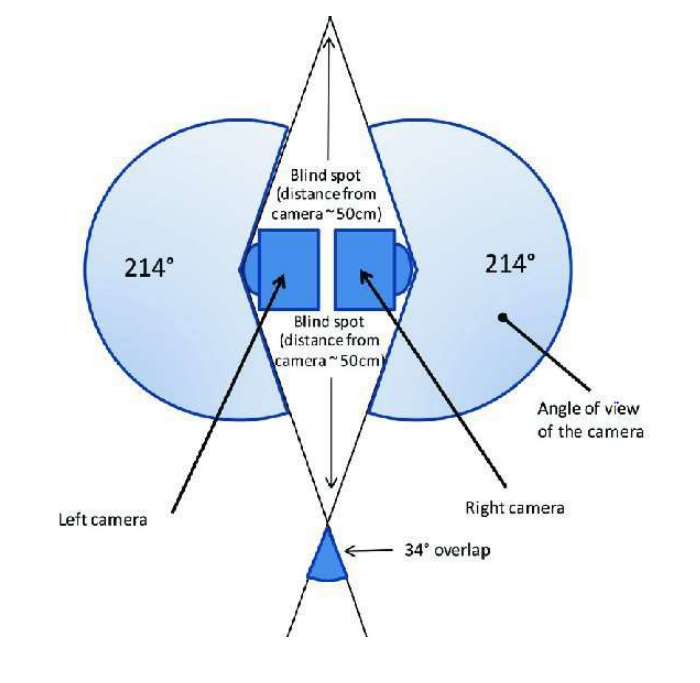
\includegraphics[width=0.9\textwidth]{Figures/360 camera coverage.PNG}
  \caption[Illustration of two camera 360 coverage]{Illustration of two camera 360 and their coverage around} \cite{karkhanis2023complete}
  \label{fig:360 camera coverage}
\end{figure}

\subsubsection{Advantages of 360 cameras}
There are several advantages to using 360-degree cameras, including:  \\
1. Immersive feeling: 360-degree cameras offer a totally spherical image, allowing viewers to see the entire scene from any angle. As a result, the viewer gets an immersive experience. This gives people the impression that they are physically present. \\
2. All-around: 360-degree cameras have numerous applications, including real estate, tourism, events, and personal use. They are useful for creating interactive video content, virtual tours, and other applications. \\
3. Expansion field of vision: A conventional camera's field of vision is limited by its lens. A 360-degree camera can capture the entire environment, providing a far wider field of view. \\
4. Virtual Reality: As virtual reality becomes more popular, 360-degree cameras are being employed to create videos on the platform. The use of 360-degree cameras greatly enhances the immersive VR experience \cite{karkhanis2023complete}. \\
\subsubsection{Constraints} 
\noindent 1. Quality: The camera's resolution, frame rate, and ISO range impact the quality of 360-degree images and videos. Lower-quality cameras may create photos or movies with reduced detail and motion blur. \\

\noindent 2. Stitching: Creating a seamless panoramic image requires stitching together several photographs or video frames. This method is time-consuming and may result in noticeable stitching flaws or inconsistencies in the final image. \\

\noindent 3. Lighting: Capturing photographs or films with a 360-degree camera can be challenging due to lighting. The camera captures light from all angles, which might cause uneven lighting or glare. \\

\noindent 4. Camera Swing: 360-degree cameras can suffer from camera wobble and motion blur due to their tiny size and lightweight design. \\

\noindent 5. Post-Production processing:Editing and post-production for 360-degree videos and photos can be time-consuming and expensive due to the need for specific software and skills. In recent advanced and newer consumer cameras, the problem of stitching and time-consumption has been substantially reduced.   \\

\noindent 6. Privacy: Capturing photographs or movies using a 360-degree camera might pose privacy problems as it captures a large field of view, potentially including individuals or private property without consent \cite{karkhanis2023complete}. But in industrial used case this item is not a consern. 



\subsection{Photogrammetry using a DSLR Camera or Smartphone}

\noindent Photogrammetry is a photographic technique that produces 3D data (measurements) from 2D images (photographs), resulting in a variety of end-results, first being a point-cloud, second is a depth map and then a mesh and finally a textured model of the object or environment with realistic color. Three main software are Metashape, Meshlab and reality-capture, by using these software you end up with a digital 3D asset.   Basically, you take a series of pictures of an object from various angles, run them through a computer application called Metashape, and you end up with a digital 3D asset. Because light and imaging methodology is so important in this process, certain objects are difficult to capture, if not impossible, to model using photogrammetry: objects with reflective or shiny surfaces, clear/transparent objects like glass, very thin objects like tree leaves, very furry or hairy things, and moving objects may sufer from these parameters\cite{PhotogrammetryWorkflowusingaDSLRCamera}.

\noindent Photogrammetry and laser scanners are now commonly used to document 3D models. Research indicates that laser scanners produce geometric data such as point-cloud and textured meshes, but photogrammetry produces higher resolution textured meshes. The high cost of laser scanners has hampered documentation practices, particularly for institutions and individuals with low means. This promotes digital photogrammetry with DSLR cameras as standard instruments although these processes are also quite time-consuming and expensive in the capture of outdoor assets or environments under sunny conditions, this also presents a set of problems due to the time takes to capture the environment or asset or the movement of the sun.Making it favourable to do such capture when it is overcast. In sunny weather , the asset or the environment tend to reflect the sun light as well as shadows which again will move due to the movement of the sun. Digital camera technology has advanced to the point where smartphones now include cameras\cite{samosir2020comparison}. \\ Smartphones are increasingly being used in photogrammetry. Smartphones are mostly used for 3D modeling because of their computer power and user-friendly software, being a cheaper alternative compare to specialized equipment such as DSLR cameras and laser scanners. Some smart phone also have integrated lidar modules. Smartphones are mostly used for rapid scanning of environments and smaller objects, enabling to capture a point-cloud and create a 3D mesh but due to inferior sensor size and lens quality the texture will suffer from less quality and resolution. \cite{Jasińska2023}. 


\begin{figure}[H]
  \centering
  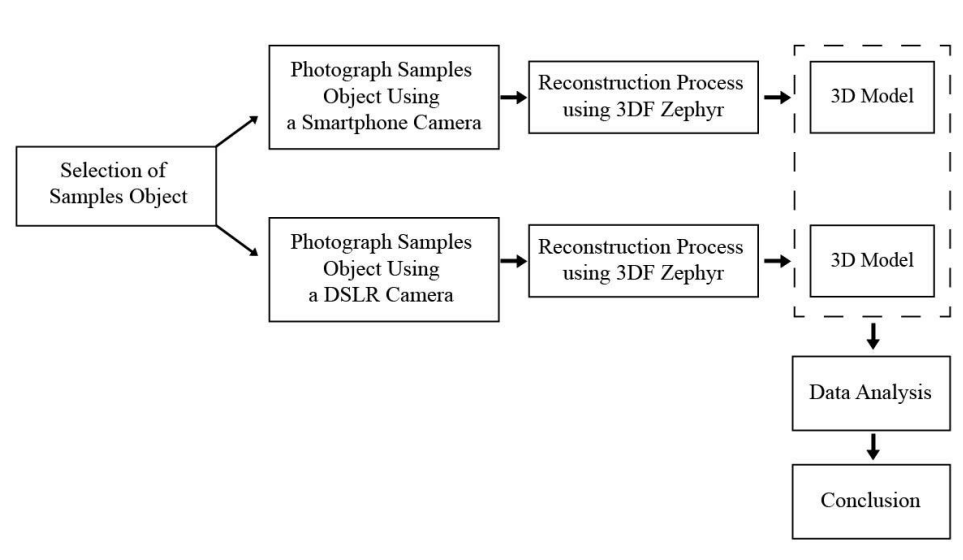
\includegraphics[width=1.01\textwidth]{Figures/Photogrammetry with DSLR Camera and Smartphone.PNG}
  \caption[Workflow of photogrammetry with DSLR camera and smartphone]{Workflow of photogrammetry with DSLR camera and smartphone} \cite{samosir2020comparison}
  \label{fig:photogrammetry with DSLR camera and smartphone}
\end{figure}

\subsection{Lidar}
Recently, the application of Light Detection and Ranging (LiDAR) technology has become widespread in various fields. The LiDAR system design has greatly improved over the years, resulting in a design that is incredibly low in cost, size, weight, and power (SWaP). Because LiDAR is lightweight and energy efficient, its use in aerial and mobile platforms has grown to allow mapping and obstacle avoidance, both of which were previously thought to be difficult. The classification of LiDAR equipment can be broad and subjective, depending on the context of use. Nonetheless, this instrument is generally classed based on the three types of information-capture functions it provides: spatial, spectral, and temporal. Every LiDAR equipment requires the ability to capture spatial information.This information is often gathered by time of flight (TOF) measurements. LiDAR systems capable of gathering spatial information are available in three varieties: one-dimensional (1D), two-dimensional (2D), and three-dimensional (3D), with optical deflecting systems used to collect 2D and 3D spatial information, respectively. The spatial data is required for creating an accurate 3D map of the environment. Creating an accurate 3D map of the environment necessitates spatial data. Yet, for applications requiring object detection, geographical information on its own is inadequate. The second class of LiDAR sensors may measure spectral information about a substance, such as laser return intensity (LRI). The term LRI refers to the reflectance caused by the interaction of the wavelength of the transmitted pulse from the LiDAR device with the targeted substance.Because the LRI is unique to a particular material type, it may be useful for determining the surface attributes of a target material. However, to avoid ambiguity in LRI readings, at least two laser wavelengths are required. Furthermore, some applications demand temporal information gathering capabilities in addition to spatial and spectral information. This can be accomplished by employing the repeated LiDAR approach\cite{raj2020survey}. Repeated LiDAR is the process of collecting temporal data from a target environment over a set length of time \cite{robin2014making}. Temporal data is critical for understanding dynamic processes like plant development and soil erosion \cite{eitel2016beyond}.\\
\subsubsection{LiDAR Architecture}
\noindent The LiDAR architecture is explained as the art of LiDAR instrumentation concerning LiDAR hardware and software \cite{FundamentalsofLidarRemoteSensing, PhysicalPictureofLidarEquation}.
A completely functional LiDAR system consists of four key subsystems: laser rangefinder, beam deflection, power management, and master controller units, as shown in Figure \ref{fig:Block diagram of LiDAR}. 
Each of these fundamental blocks is equally essential, and a malfunction in any of these subsystems could lead to a decrease in the LiDAR system’s functionality. However, without the beam deflection subsystem, the LiDAR might still work as a 1D LiDAR, also known as a laser range finder (LRF)\cite{raj2020survey}.

\begin{figure}[H]
  \centering
  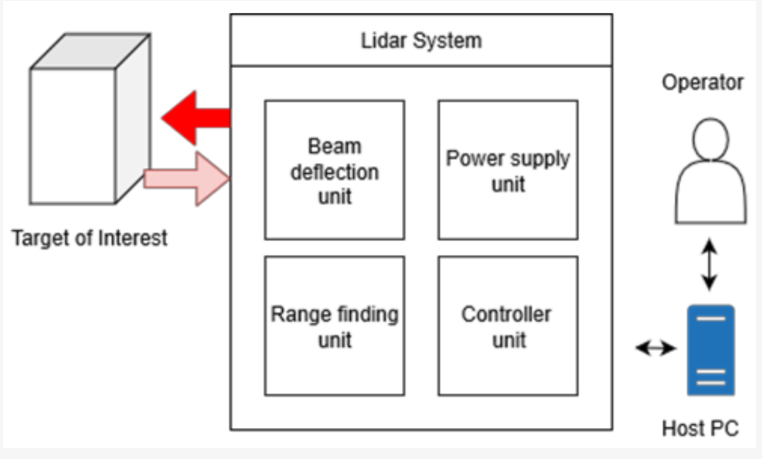
\includegraphics[width=0.9\textwidth]{Figures/Block diagram of LiDAR system.PNG}
  \caption[Illustration Block diagram of LiDAR]{Illustration of Block diagram of LiDAR} \cite{raj2020survey}
  \label{fig:Block diagram of LiDAR}
\end{figure}

\subsubsection{LiDAR Specifications}
The LiDAR scanner parameters are critical information for a developer to select the best solution for his application. It can be divided down into four tiers, as shown in Figure \ref{fig:Hierarchy of LiDAR specifications}. 
The first parameters in the hierarchy include information about ranging, such as maximum and minimum detection range, resolution, accuracy, and update frequency. The second specification in the hierarchy is connected to physical aspects such as size, weight, and power consumption, which can be found in a product manual. These criteria are critical for applications involving mobile or aerial platforms where size, weight, and power may be limited. Because LiDAR uses lasers, information about the wavelength, power emitted, and laser class is provided in the specs to ensure safety compliance.Examples of optical specifications mentioned in product manuals include lens focal length and beam divergence. The specs provided thus far only define the properties of 1D LIDAR. In the case of scanning LiDAR, extra parameters about beam deflection motion are required. This specification defines characteristics such as field of vision (FOV), angular resolution, response time, and number of scan points \cite{raj2020survey}.
\begin{figure}[H]
  \centering
  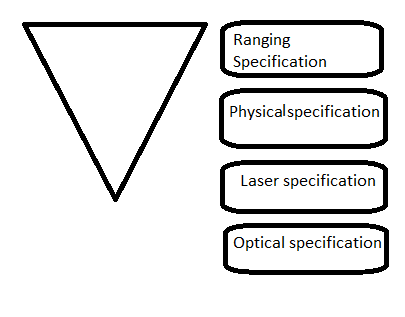
\includegraphics[width=0.8\textwidth]{Figures/Hierarchy of LiDAR specifications.png}
  \caption[Illustration of Hierarchy of LiDAR specifications]{Illustration of Hierarchy of LiDAR specifications} \cite{raj2020survey}
  \label{fig:Hierarchy of LiDAR specifications}
\end{figure}
\subsubsection{Used Case of LiDAR and 3D Ship Model for Battle Damage Assessment in a Frigate}


The static detonation training exercise in late March 2022, during which an explosive charge was placed aboard the ship with the intention of harming it, and the future evolution are essential components of a lidar-focused megaproject financed by the Naval Innovative Science and Engineering (NISE) program. As part of the project, different combat centers collaborate to create 3D models of complete ships from lidar scans, with the goal of expanding the models' use in battle damage assessment and repair, installation and modernization, and other fleet applications \cite{defenseadvancement}. \\
This technology allows for the speedy capture of damage, overlaying it on the baseline model, precisely documenting the state, and then sharing the data with the greater community to help engineers make decisions. The initiative comes as lidar scanning tools become more accessible and affordable. By leveraging technology to create more 3D ship models, stakeholders and partners hope to reduce the need for engineering teams to travel to ships, enable more remote support such as virtual ship checks, and reduce response times to casualties and maintenance issues that the fleet encounters at sea. Because it is possible to send the 3D model to the people but not the ship. Lidar examines an object in three dimensions by bouncing laser beams off of it and timing how long they take to return. The system can record a massive network, or cloud, of data points and stitch together scans from various angles to produce a millimeter-accurate 3D digital image of the object \cite{LidarSolutionforship, deems2013lidar}. The most recent lidar scanning equipment can also collect images and overlay them on the data point cloud, resulting in a more realistic model. \\
More accurate installation drawings, for example, could aid in the avoidance of unexpected hurdles and delays during ship construction. Lidar scans can generate 3D models of ships that are precise to the millimeter. Installation and upgrade teams can use these models to measure parts of the ship before embarking to install equipment. In this digital environment, it is feasible to collect exact measurements between components as well as calculate distances between bulkheads and equipment. Designers can ensure that doors and cabinets open properly.  Engineers are looking for obstacles to our installation that need to be moved or planned around. Due to high expenses of this method, it is better to involve interested-parties who works on different areas of a ship \cite{defenseadvancement}. 
\subsubsection{Full Ship Scan}
In 2020, the complete interior and exterior of the amphibious transport dock USS San Diego (LPD 22) were lidar-scanned. The end result was the first full-size 3D digital model of an LPD-class vessel. Scanning a complete ship may appear expensive due to the massive data collection and processing required. Approximately the course of roughly two months, the team that scanned the USS San Diego collected approximately 7,000 unique scans from various points within and outside of the mammoth warship. Full-ship scanning gains even more value when its application spreads across other fighting centers. In other words, the cost per user decreases as the number of stakeholders using the data collection increases\cite{defenseadvancement}. 
\subsubsection{Combination of Photogrammetry and LiDAR in Ship Damage Assessment}
Ships can sustain various sorts of damage, including structural damage from weapons attacks, collisions, corrosion \cite{aijazi2016detecting}, and exceeding operational loads. Normally, damage assessment inspectors must visit to the ship to assess the damage, take photos, and write a report. To respond to casualties more efficiently and precisely, Nahshon realized the potential of comparing a ship's "healthy" pre-casualty 3D model to its damaged condition. Unmanned aircraft systems (UAS), commonly known as drones, make it easier to acquire photographs and videos of damaged regions aboard ships. Photogrammetry, a sort of 3D scanning, involves stitching together footage from a UAS to create a 3D depiction of the damaged region. This updated model might then be compared to the lidar scan's pre-casualty healthy model to get a more accurate picture of the damage \cite{defenseadvancement}. 

\subsection{Preface for Simultaneous Localization and Mapping (SLAM)}
SLAM, or simultaneous localization and mapping, is a subject in mobile robotics and artificial intelligence that has been extensively studied for over two decades. Scientists employ many approaches to enhance the autonomy and self-exploration of robot navigation. Autonomous robots are intelligent systems that can navigate their surroundings without human intervention. To navigate successfully, robots must have a strong grasp of their surroundings and accurately track their whereabouts.The robot's location, also known as its state, determines its pose, position, and orientation on the map. The map depicts the environment's elements, such as walls, barriers, and landmarks. A map is necessary for mobile robots to navigate and plan their paths. Localization refers to the process of predicting a robot's position in recognized environments using sensor data and a pre-defined map \cite{thrun2002probabilistic}. 
Numerous studies have examined the localization problem across various criteria and situations. A fully intelligent mobile robot should be able to explore unfamiliar environments without relying on a pre-existing map.For indoor applications where GPS is not available, a reliable mechanism for estimating the robot's stance is necessary.However, the popularity of applications that erase user-created maps has made mapping necessary for mobile robots. The SLAM technique is effective for solving problems when prior knowledge or maps are unavailable or undesirable. SLAM techniques create a map of the environment without prior information and locate the robot without human input. It allows robots to operate without relying on ad-hoc localization infrastructure. Robots require a map (e.g., identifiable landmarks) to rectify misalignments caused by uncertainties in their movements, such as drifts and dead reckoning.Future SLAM systems should provide autonomous navigation in all environments, including indoors, outdoors, underwater, and air, with minimal estimation errors, long-lasting mapping, and low-power and computing costs. Simplicity is also important \cite{Taheri2021}. 
\subsubsection{Simultaneous Localization and Mapping (SLAM)}
SLAM solution strategies have advanced rapidly over the last two decades. SLAM algorithms utilize numerous sensors, including ultrasonic sensors, laser scanners, and RGB cameras, to estimate robot stance and create two- or three-dimensional maps. The 2D SLAM challenge with rangefinders is considered solved \cite{li2016real}, however, this assertion is incorrect, as advances in accuracy, speed, and massive data processing are needed for 2-D SLAM problems. Unmanned systems, including UAVs, self-driving cars, building inspections, surveillance, and underwater SLAM, face challenges in outdoor, unstable, and dynamic environments. Furthermore, every technique has room for improvement. Most SLAM failures are caused by perception instability or uncertainty. SLAM includes two parts: localization and mapping. Initially, SLAM technology focused on mapping and localization individually. Modern studies recognized that localization and mapping are very interdependent. The map is necessary for accurate localization, whereas localization is crucial for mapping. As a result, the word is known as a ''Chicken and egg'' question. Classical SLAM algorithms estimate poses and maps collaboratively. However, more sophisticated systems view localization and mapping as two simultaneous operations, resulting in the well-known simultaneous Tracking and Mapping (PTAM) \cite{klein2007parallel,Taheri2021}. 
In robotics, odometry is the estimation of a robot's motion over time using motion sensors such as wheel encoders. Odometry models using various sensors, including Visual Odometry (VO) with cameras, have advanced significantly. Improving the precision of the odometry model reduces uncertainty in robot navigation and improves mapping. Mapping is significant in three fundamental aspects: \\
1. Maps provide path planning and obstacle avoidance. \\
2. Many mobile robotics applications aim to create maps.\\
3. The durability and accuracy of localization are highly dependent on mapping accuracy.\\
Loop closure is a key component of mapping, allowing robots to recognize visited locations and optimize their estimated poses. The loop closure significantly decreases drifts and allows the robot to adjust for odometry inaccuracies. Visual odometry approaches often incorporate mapping, but the map may not be relevant to path planning or local task execution. SLAM varies from modern odometry models by optimizing the global map and closing the loop \cite{cadena2016past}. Positioning is an important aspect of SLAM. There are two approaches to tackling positioning difficulties: probabilistic and non-probabilistic. Probabilistic approaches are often used for categorization. Probability approaches rely on Bayesian estimates, primarily using Particle Filters (PF) and Kalman Filters (KF). Gaussian distributions are used for system inputs, motion model output, observed data, observation outputs, and state noise. KF provides the most accurate assessment of the robot pose \cite{yavuz2009simultaneous}.
The KF-based SLAM approach is popular due to its simplicity of implementation and advantage in convergence. However, it lacks a loop closure and has issues with data association, which can lead to system failure. KF is typically applied to linear systems, while nonlinear systems are more common in practice. Nonlinear systems can be linearized with the Extended Kalman Filter (EKF) and first-order Taylor expansion \cite{julier2001counter}.\\
An overview of a standard SLAM algorithm based on the EKF is provided below: \cite{Taheri2021}\\
\noindent 1. The elementary map is created using initial sensory input.\\
2. Characterizes the robot's beginning stance and surrounding locations.\\
3. The robot updates its location and map information as it moves around.\\
4. New landmarks are derived from the revised map.\\
5. The robot recognizes new landmarks and adjusts its location accordingly.\\
6. The robot follows a new path based on the updated map until it reaches its destination.\\
 Figure \ref{fig:Feature based slam} depicts a common block diagram for a feature-based SLAM issue \cite{leonard2012directed}. 
\begin{figure}[H]
  \centering
  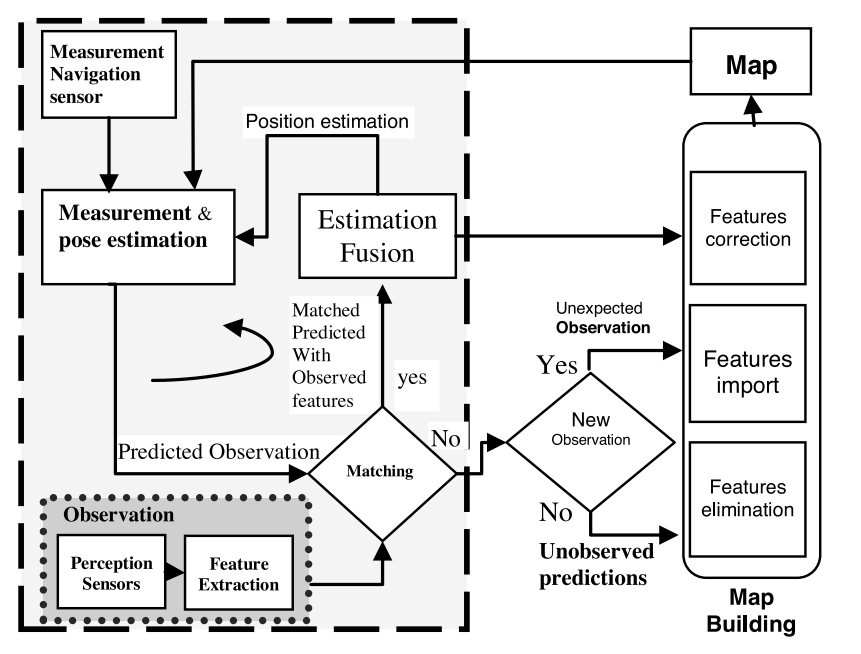
\includegraphics[width=0.9\textwidth]{Figures/Feature based slam.PNG}
  \caption[Illustration of Feature based slam]{Illustration of Feature based slam} \cite{leonard2012directed}
  \label{fig:Feature based slam}
\end{figure}

\subsection{Visual SLAM}
Simultaneous Localization and Mapping (SLAM) captures the 3D structure of an unfamiliar environment while also tracking sensor mobility. This technique was initially presented for autonomous control of robots in robotics \cite{chatila1985position}. SLAM-based applications have expanded to include computer vision, online 3D modeling, AR visualization, and self-driving cars \cite{durrant2006simultaneous,bailey2006simultaneous, stachniss2016simultaneous,aulinas2008slam}. In this section, we talked about  SLAM employing cameras due to their simple sensor design and higher technological hurdles compared to other methods. Visual SLAM (vSLAM) is a technology that relies solely on visual information as input. vSLAM algorithms have been widely used in computer vision, robotics, and augmented reality \cite{billinghurst2015survey}. These methods are ideal for estimating camera poses in AR systems with simple configurations, such as camera-mounted tablets or smartphones. Real-time response is a key requirement in AR systems because it allows real and virtual items to be smoothly and interactively merged.The use of vSLAM algorithms is not limited to AR systems. It has applications in robotics, such as unmanned autonomous vehicles (UAVs). In general, vSLAM is more technically challenging than other sensor-based SLAMs since cameras can capture less visual information from a smaller field of view than 360° laser sensing, which is commonly employed in robotics. Camera postures must be continuously calculated from such data, while the 3D structure of an unknown environment is recreated at the same time. In the 2000s, the early work on vSLAM with a monocular camera focused on tracking and mapping feature points. This is referred to as "feature-based approach." To deal with texture-less or feature-less surroundings, vSLAM has been developed that works without detecting feature points and instead tracks and maps the entire image. This is known as "direct approach". With the introduction of low-cost RGB-D sensors such as the Microsoft Kinect, vSLAM algorithms that use both a monocular picture and its depth have been developed  \cite{Taketomi2017}. 
\begin{figure}[H]
  \centering
  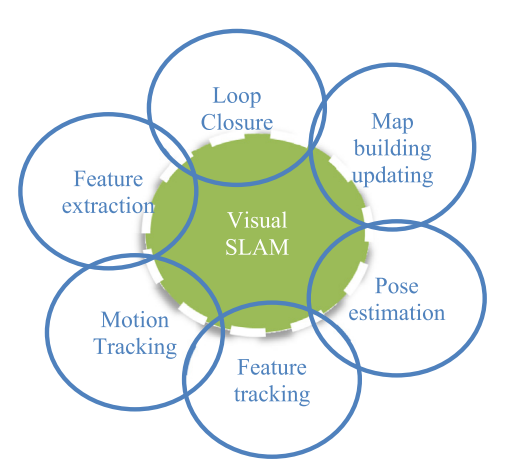
\includegraphics[width=0.6\textwidth]{Figures/Visual SLAM Components.PNG}
  \caption[Illustration of Visual SLAM Components]{Illustration of Visual SLAM Components} \cite{Taheri2021}
  \label{fig:Visual SLAM Components}
\end{figure}


\subsection{Neural Radiance Field (NeRF)}
Synthesizing new viewpoints on a scene from a small number of gathered photographs is a long-standing computer vision problem that is necessary for many AR and VR applications.
Classic techniques, such as structure-from-motion or image-based rendering, have been employed to tackle this problem 
 \cite{martin2021nerf,shum2008image}. Neural rendering techniques, which incorporate learning modules into a 3D geometric context and train them to rebuild observed images, have led to tremendous development in this discipline. The Neural Radiance Fields (NeRF) technique uses neural network weights to model a scene's radiance and density \cite{mildenhall2021nerf}.
 View synthesis involves creating fresh perspectives of a scene using input photos and camera poses. Accurately handling complicated geometry and material reflectance attributes is crucial for creating lifelike outputs from different perspectives. 
Several scene modeling and rendering solutions have been proposed to address this issue, but none have yet achieved photorealistic quality across a large camera baseline \cite{mildenhall2021nerf}.
NeRF is only effective in controlled conditions where the scene is taken quickly with continuous illumination and static material. Moving objects or varying illumination severely reduce NeRF's performance, as demonstrated \cite{martin2021nerf}. Mildenhall and his group provides a cutting-edge strategy for creating innovative views of complicated scenes by maximizing a continuous volumetric scene function using sparse input views. Their algorithm uses a nonconvolutional deep network to represent a scene. It takes a single continuous 5D coordinate (x, y, z) and viewing direction  \(\theta,\phi\)\ as input and outputs volume density and view-dependent radiance. They create views by querying 5D coordinates along camera rays and use volume rendering algorithms to project colors and densities into a picture. Volume rendering is naturally differentiable, therefore optimizing the representation requires only a set of photos with known camera postures. Mildenhall explains how to optimize neural radiance fields to create photorealistic views of complex scenes and the results outperform previous work on neural rendering and view synthesis \cite{mildenhall2021nerf}. 
In Figure \ref{fig:Optimized NeRF} it is shown the schematic of optimized method by Mildenhall.
\begin{figure}[H]
  \centering
  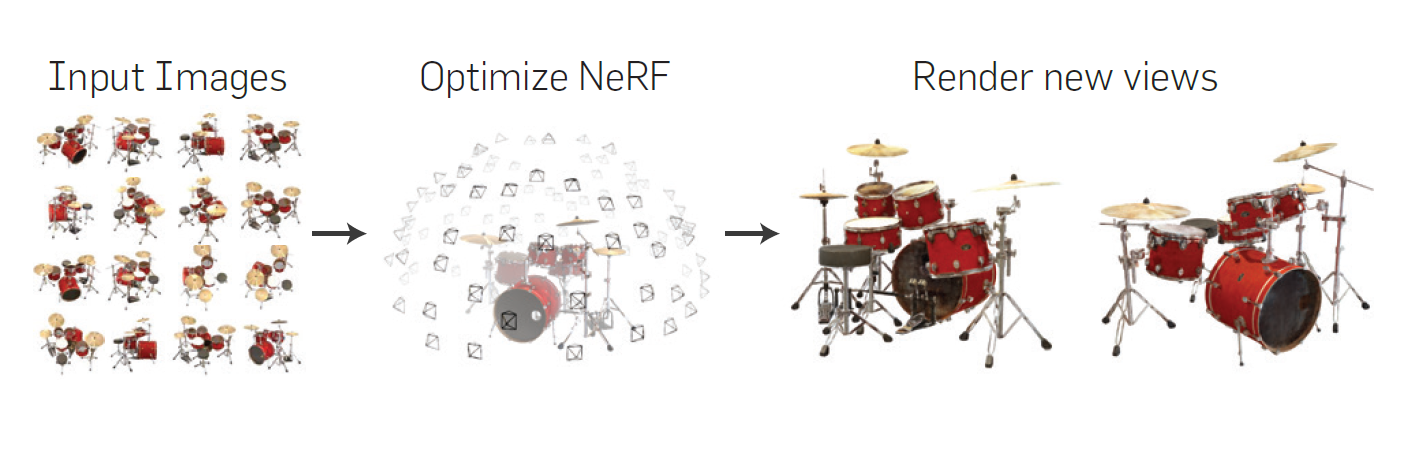
\includegraphics[width=0.9\textwidth]{Figures/Optimized NeRF.PNG}
  \caption[Illustration of Optimized NeRF]{This image illustrates a technique for refining a continuous 5D neural radiance field representation (comprising volume density and view-dependent color at each continuous point) of a scene, using a sequence of input photos. It employs volume rendering algorithms to collect samples of this scene representation along rays, enabling the scene to be portrayed from any viewpoint. Displayed below are 100 input views of the synthetic Drums scene, randomly selected from a surrounding sphere, followed by two novel views generated using the optimized NeRF representation \cite{mildenhall2021nerf}.}
  \label{fig:Optimized NeRF}
\end{figure}

\subsection{3D Gaussian Splatting and Compare With NeRF}
Neural radiance fields (NeRF) revolutionized computer graphics and 3D scene reconstruction by allowing for novel-view synthesis \cite{mildenhall2021nerf, avidan1997novel}. NeRF, based on deep learning and computer vision, can generate lifelike scenarios from sparse input views, creating a new paradigm in image synthesis.
However, NeRF, like any new technology, has faced hurdles and limits, particularly in terms of computing efficiency and control. 3D Gaussian splatting (3D GS) is a paradigm-shifting approach that redefines scene representation and rendering, rather than just incremental improvements \cite{kerbl20233d}. Prior to NeRF, novel-view synthesis focused on light fields and basic scene reconstruction algorithms \cite{gortler2023lumigraph, buehler2001unstructured}. Initial approaches were hampered by their reliance on deep sampling and structured capture, which made it difficult to handle complicated scenes and lighting. Structure-from-motion (SfM) and multi-view stereo (MVS) techniques improved 3D scene reconstruction and paved the way for advanced view synthesis
 \cite{snavely2006photo, goesele2007multi}. NeRF marks a significant advancement in this field. NeRF uses neural networks to map spatial data to colors and density. NeRF's success relied on its capacity to provide continuous, volumetric scene function, resulting in remarkable detail and realism. However, the implementation came at a cost. NeRF approaches were computationally costly, necessitating lengthy training and significant rendering resources, particularly for high-resolution results \cite{chen2022tensorf,garbin2021fastnerf,reiser2021kilonerf,takikawa2021neural, barron2022mip, muller2022instant}. 3D GS arose in response to these issues. Although NeRF excelled at creating photo realistic images, there was a growing demand for quicker and more efficient rendering methods, particularly for real-time applications. 3D GS introduced a revolutionary scene representation technique that employs millions of 3D Gaussian. Compared to implicit coordinate-based models, 3D GS uses explicit representations and parallelized workflows for efficient calculation and rendering \cite{mildenhall2021nerf,henzler2019escaping, sitzmann2019deepvoxels}.3D GS innovates by combining differentiable pipelines with point-based rendering approaches \cite{pfister2000surfels,wiles2020synsin}. Using learnable 3D Gaussians in scene representation preserves the desirable properties of continuous volumetric radiance fields for high-quality image synthesis while avoiding the computational overhead of rendering in empty space, which is a common drawback in traditional NeRF methods \cite{chen2024survey}. The emergence of 3D GS marks a significant shift in scene representation and rendering in computer graphics, beyond only technical advancements.
3D GS allows for real-time rendering without sacrificing visual quality, making it suitable for various applications such as virtual reality, augmented reality, and real-time cinematic rendering \cite{kalkofen2008comprehensible,patney2016towards,albert2017latency}. This technique has the potential to improve existing applications and enable new ones that were previously not possible due to computational constraints. Furthermore, 3D GS's explicit scene representation provides unparalleled control over complicated scenes with intricate geometry and changing lighting conditions \cite{chabra2020deep,wang2021learning}. 3D GS's control and edit-ability, along with its efficient rendering process, make it a transformational force in defining future improvements in the industry \cite{chen2024survey}.



\subsection{Image Segmentation}
Image segmentation is a popular research subject in computer vision, serving as the foundation for pattern recognition and picture understanding. Image segmentation has applications in various fields, including driver-less vehicles \cite{kabiraj2023number}, medical technology \cite{zhao2021voxelembed, jin2020deep}, search engines \cite{yao2021compound}, industrial inspection, and augmented reality. 
Image segmentation is a crucial step in comprehending natural scenes and is a popular study topic in image processing. It involves splitting a picture into meaningful, non-overlapping areas.Image segmentation involves three stages: traditional segmentation, collaborative segmentation, and semantic segmentation using deep learning as you can see in Figure \ref{fig:Categories of Image segmentation}. Image segmentation identifies areas of interest (ROIs) based on various attributes in an image. Humans perceive these zones as meaningful and non-overlapping. Image segmentation presents two challenges: (1) defining "meaningful regions" due to uncertainty in visual perception and human comprehension, making it an ill-posed problem; and (2) effectively representing objects in an image. Pixels in digital photos can be combined to create bigger sets based on color, texture, and other characteristics. These are known as "pixel sets" or "superpixels". Low-level picture features indicate local attributes, but obtaining global information (e.g., shape and position) from them is challenging.
\cite{yu2023techniques}

 
\begin{figure}[H]
  \centering
  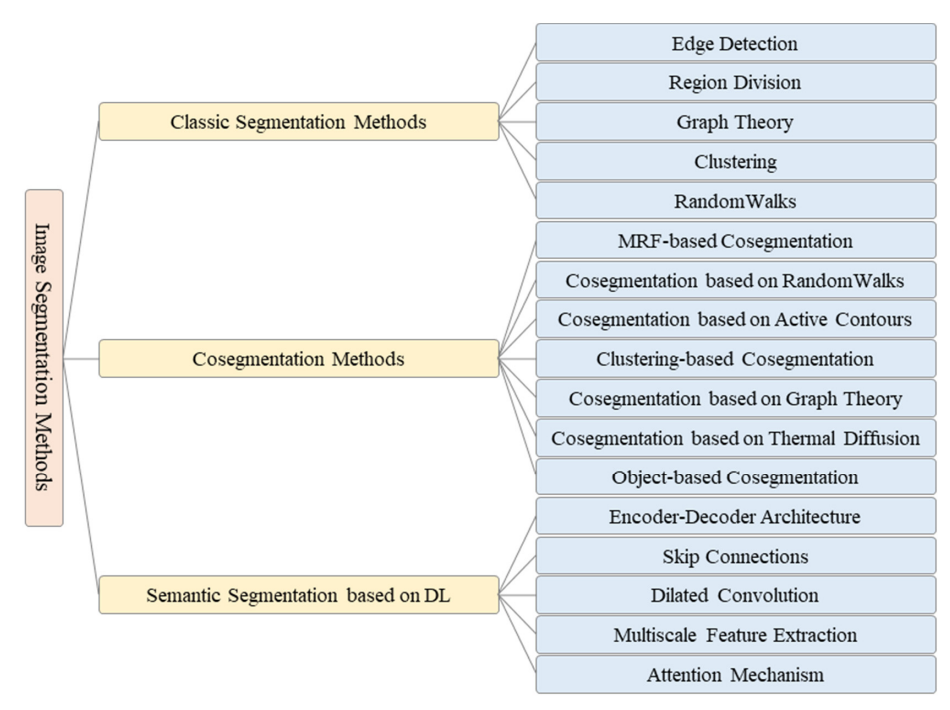
\includegraphics[width=0.9\textwidth]{Figures/categories of image segmentation method.PNG}
  \caption[Illustration of categories of image segmentation ]{This picture shows categories of image segmentation \cite{yu2023techniques}.}
  \label{fig:Categories of Image segmentation}
\end{figure}

\subsection{3D or Video Segmentation}
3D geometric data can be represented as point clouds, meshes, voxel grids, depth maps, parametric models, or RGB-D images. Segmenting 3D data can be hard, with several techniques available for different representations. Video sequences can be considered 3D data, as time is a third dimension. As still-image segmentation techniques improve, video segmentation is becoming increasingly popular.
Using still-image segmentation methods on video frames might be computationally expensive and fail to capture the temporal continuity of the content. Segmenting 3D/video data entails assigning labels to each minimal unit. Minimum unit can be a voxel, point, mesh or pixel within a video frame.In addition to practical picture segmentation applications, 3D segmentation is used in robotics and augmented/virtual reality \cite{wang2022comprehensive}. 





\subsubsection{Voxel-based Semantic Segmentation}
Deep learning has achieved significant success in picture, audio, and text recognition. However, few studies have investigated 3D large-scale point cloud classification. Unlike pictures, where the spatial relationships between pixels can be captured by sliding windows, the points in a point cloud are unstructured and the density is uneven. Parsing a 3D point cloud with noise, outliers, and under-sampling can be challenging. Liu \cite{liu20173dcnn} proposed a method called  3DCNN-DQN-RNN is intended to meet this difficulty. The model includes 3D convolutional neural network (3DCNN), Deep Q-Network (DQN), and residual recurrent neural network (RNN). The 3DCNN network learns visual, spatial, and contextual features from point cloud data at various scales, resulting in a 3D feature representation. The DQN uses trial-and-error to localize class objects through an eye window. The 3DCNN calculates a reward based on the eye window points, capturing significant features quickly. The eye window points' colors and coordinates are combined with the 3DCNN feature representation to create an input vector. This vector is then fed into the RNN to generate the final class labels. In the Figure \ref{fig:Liu Framework approach} the framework of this methods is shown. 
\begin{figure}[H]
  \centering
  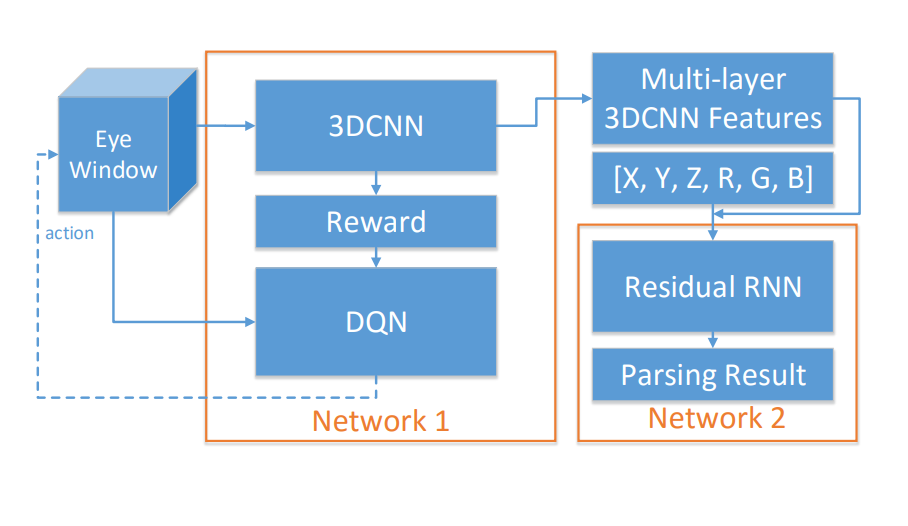
\includegraphics[width=0.9\textwidth]{Figures/Framework of Liu proposed approach.PNG}
  \caption[Illustration of Liu framework ]{This picture shows Liu framework approach that (X, Y, Z) and (R, G, B) representing 3D coordinate and RGB colors of each point in the original point cloud. \cite{liu20173dcnn}.}
  \label{fig:Liu Framework approach}
\end{figure}

\subsubsection{Point Cloud-based Semantic Segmentation}
3D point cloud segmentation divides point clouds into homogeneous zones, where points have similar attributes. Segmenting point cloud data is problematic due to significant redundancy, inconsistent sample density, and lack of explicit structure. This topic has multiple applications in robotics, including intelligent vehicles, autonomous mapping, and navigation \cite{nguyen20133d}. To handle point clouds, CNNs cannot be used directly and must be converted to other forms or adjusted to allow for data permutations.  Distances between points can help segmentation models identify objects or clusters in 3D space due to their variability \cite{wang2022comprehensive}. 

\begin{figure}[H]
  \centering
  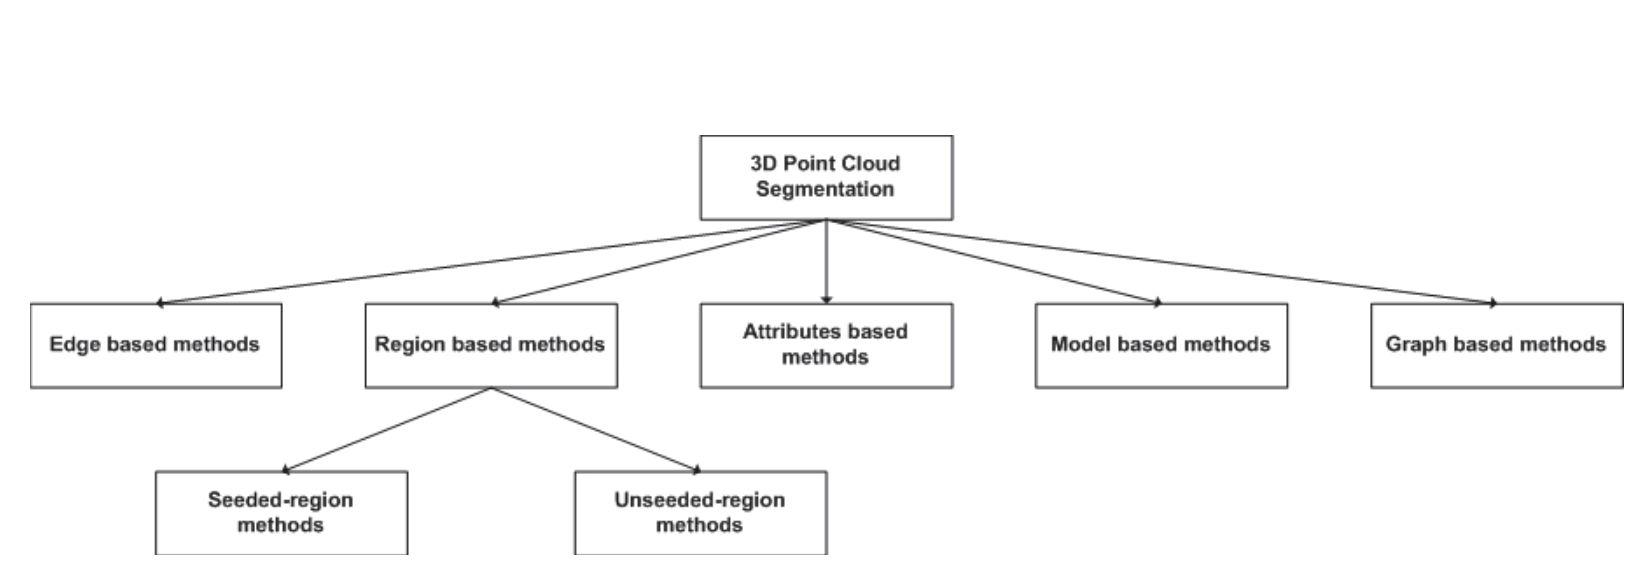
\includegraphics[width= 1.0\textwidth]{Figures/Taxonomy of 3D point cloud Segmentation methods.PNG}
  \caption[Illustration of Taxonomy of 3D point cloud Segmentation methods ]{This picture shows Taxonomy of 3D point cloud Segmentation methods \cite{nguyen20133d}.}
  \label{fig:Taxonomy of 3D point cloud Segmentation methods}
\end{figure}
 
\subsubsection{Semantic Segmentation by Robots}

Robots require a thorough understanding of their surroundings before interacting with the world. The accuracy with which a robot performs a task, navigates, or communicates is highly dependent on how well it understands its surroundings. Understanding context is vital for operating safely in varied situations \cite{premebida2018intelligent}. Accurately interpreting the surroundings is tough, particularly in complex and dynamic metropolitan environments. In these situations, robots are expected to complete their tasks perfectly despite encountering a variety of agents and objects. The process becomes more challenging when the appearance of the scene changes with lighting and weather conditions \cite{valada2020self}. Scene understanding in robotics entails identifying, localizing, and describing the elements that make up the environment, as well as their characteristics and dynamics. Because of the potential benefits for a wide range of applications, research on novel automatic scene interpretation systems has increased significantly during the last ten years. Advances in deep learning, open-source datasets, and increased computational resources have led to rapid improvements in scene interpretation approaches \cite{premebida2018intelligent}. 
visual classification is a prime example of technological advancements in determining visual content. This classification task's output can be considered a high-level representation of the scene, allowing for the identification of the numerous items present by assigning them a class label. Object detection is a mid-level feature that uses bounding boxes to classify and localize items in a picture, providing additional details. Although this assignment provides a more detailed representation of the scene, it is still unable to offer critical information or item properties such as object shape. Object segmentation is a related task that provides the shape of an object within a bounding box based on its segmented boundaries. Figure \ref{fig:From input image to semantic segmentation} shows an overview of various perceptive tasks\cite{hurtado2022semantic}.

\begin{figure}[H]
  \centering
  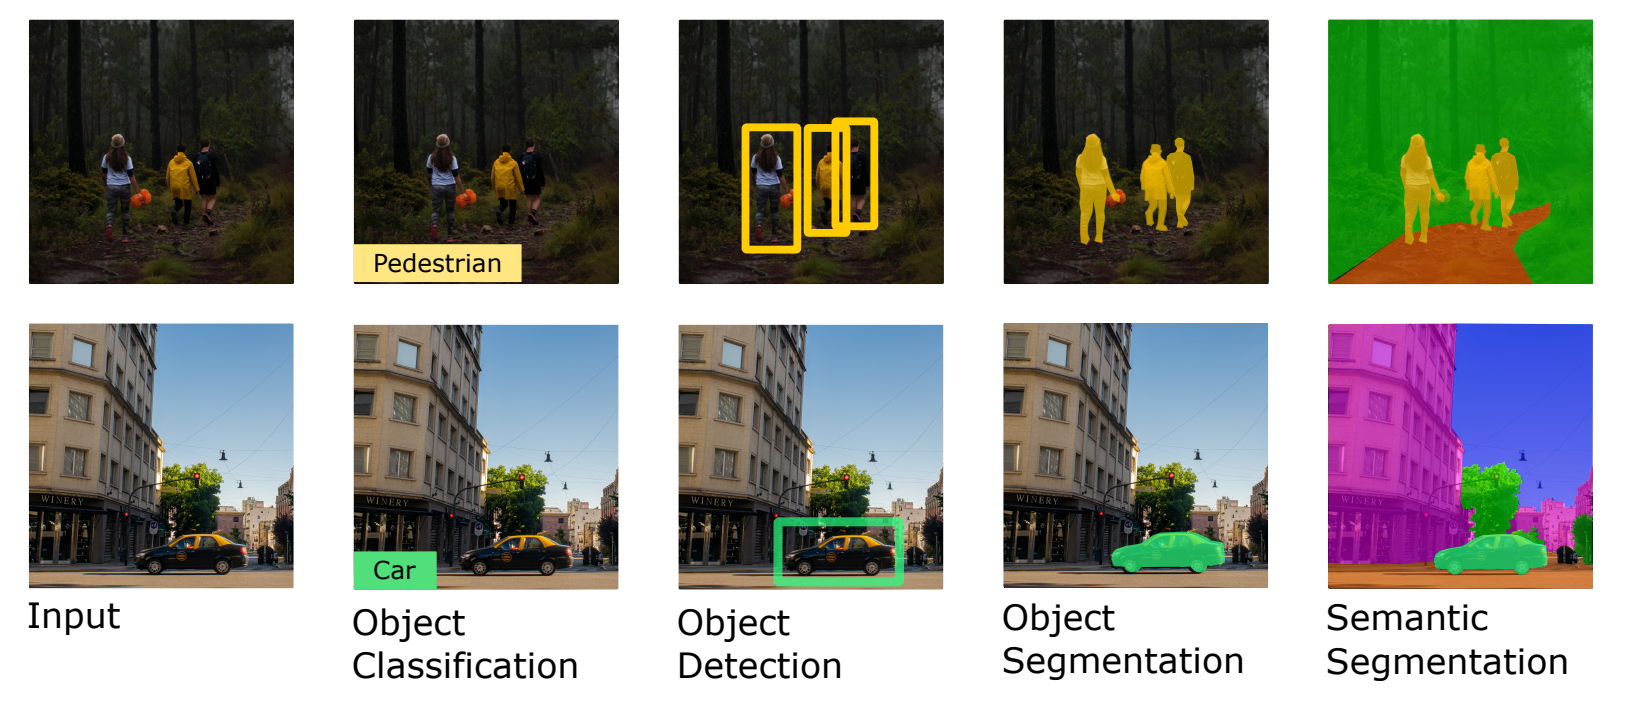
\includegraphics[width= 1.0\textwidth]{Figures/From input image to semantic segmentation.PNG}
  \caption[Illustration of From Input Image to Semantic Segmentation ]{In this picture each row displays an example of an input image and its matching output for various scene interpretation tasks. Object classification determines "what" items are in the image, whereas object detection predicts "where" they are, and object segmentation produces a mask indicating the shape of the object. Semantic segmentation enhances the input image by predicting the labels for all pixels, including the background.
 \cite{hurtado2022semantic}}
  \label{fig:From input image to semantic segmentation}
\end{figure}












